\documentclass[10pt, a4paper]{article}
\usepackage[margin=1.5cm]{geometry}
\usepackage{graphicx}

\title{Appunti Tecnologie Open-Source}
\date{A.A. 2020/2021}
\author{Michele Veronesi}

\begin{document}
\maketitle
\tableofcontents

\newpage
\section{Issue Tracking System - ITS}
\textit{Issue}: criticità, evento da gestire\\
\textit{Tracking}: registrare, lasciare traccia
\subsection{Definizione}
Un Issue Tracking System (ITS) è un pacchetto software che gestisce e mantiene una lista di criticità (issue), come richiesto da un'organizzazione.\\
Questo tipo di sistema è spesso usato nei call center di supporto delle aziende per creare, aggiornare e risolvere i problemi segnalati dai clienti o dagli impiegati.\\
In sostanza, è uno strumento che semplifica la gestione del processo di sviluppo e di change management attraverso la gestione di attività diverse (Work item) come: analisi requisiti, sviluppo, test,  bug, release, deploy, change request...\\
Ogni singola "attività minima" (work item) del progetto è gestita mediante un workflow e mantenuta all'interno di un'unica piattaforma e un'unica repository.

\subsection{A cosa serve}
\begin{itemize}
\item Condividere le informazioni tra team di sviluppo, project manager e cliente, infatti offre un unico repository in cui trovare le informazioni e un sistema di notifica.
\item Implementare il processo di misurazione della qualità del progetto
\item Avere un'istantanea dello stato del progetto: attività da fare, in corso d'opera, completate.
\item Decidere cosa rilasciare e quando rilasciare: i work item possono essere assegnati ad una versione
\item Assegnare una priorità alle attività
\item Avere una chiara assegnazione delle responsabilità sulle attività: ogni work item riporta incaricato e assegnatario
\item Tiene la memoria storica di tutti i cambiamenti
\end{itemize}

\subsection{Workflow}
Il workflow è un insieme di stati e transizioni che un work item attraversa durante il suo ciclo di vita. Viene associato ad un progetto e ad uno o più tipi di work item. Permette di registrare tutte le transizioni e i cambi di stato.

\subsection{Collegamenti}
Permettono di mettere in relazione vari work item, anche di differenti tipi (attività, sotto-attività, requisiti, casi di test, ...), sono bidirezionali e vengono registrati come criterio di ricerca. Questo permette di verificare la presenza o meno di relazione tra i work item (per esempio vedere se un requisito è coperto da casi di test).

\subsection{Funzionalità}
\begin{itemize}
\item Ricerca avanzata dei work item
\item Salvataggio di ricerche
\item Esportazione
\item Notifiche
\item Bacheche o board
\item Reporting
\item Dashboard
\item Definizione di Road map e Release Notes
\item Integrazione con il Source code management
\item Integrazione con l’ambiente di sviluppo
\end{itemize}

\subsubsection*{Filtri}
I filtri permettono di ricercare i work item in base ai campi, possono essere salvati per facilitare le ricerche più recenti, i risultati possono essere esportati e \underline{sono la base per creare report, board e dashboard}.

\subsubsection*{Board o bacheche}
Permette di visualizzare i work item di uno o più progetti, offrendo un modo flessibile e interattivo di visualizzazione, gestione e visualizzare dei dati di sintesi sulle attività in corso.\\
È configurata e visualizza i work item ricercati con un filtro.\\
Permette di interagire velocemente con i work items (avanzare di stato, modificare alcuni campi).

\subsection{Configurazione e utilizzo}
\begin{enumerate}
\item Identificare i processi richiesti per la gestione del progetto: vincoli imposti dal cliente, procedure e best practices definiti dai framework di qualità presenti in azienda o imposti dal cliente.
\item Identificare e configurare gli strumenti che permettono di implementare i processi (ITS): identificazione e definizione dei tipi, dei campi custom, dei work flow e dei collegamenti che ci permettono di tracciare le informazioni richieste dal processo.
\end{enumerate}

\begin{itemize}
\item Il manager del ITS: 
	\begin{itemize}
	\item crea un nuovo progetto
	\item definisce il processo da seguire (tipi di work item, campi custom, work flow, collegamenti), seleziona il modello di stima, differenti board e report per processo
	\item Aggiunge gli utenti e assegna ruoli/permessi
	\end{itemize}
	
\item Il manager (capo progetto):
	\begin{itemize}
	\item Definisce le versioni (release)
	\item Definisce le componenti del progetto
	\item Definisce i lavori da svolgere (backlog): priorità, assegnatario e stima
	\item Definisce la prima iterazione
	\item Monitora l’avanzamento e il completamento delle attività (filtri, board, dashboard, report)
	\item Definisce le nuove versioni
	\item Definisce le nuove iterazioni
	\item Definisce, aggiorna e monitora le attività (priorità, verifica stima/consuntivo)
	\item Produce i report richiesti dal cliente (p.es. Calcolo SLA, release log, ...)
	\end{itemize}	 
	
\item Gli utenti (il team di sviluppo):
	\begin{itemize}
	\item Ricevono le notifiche dei work item assegnati
	\item Selezionano i work item in base alle priorità
	\item Avviano e completano la lavorazione: avanzano gli stati del workflow, aggiornano la stima a finire, registrano il tempo impiegato
	\item Completano tutte le attività presenti nell'iterazione
	\item Effettuano il rilascio
	\end{itemize}
\end{itemize}

\subsection{Vantaggi ITS}
\begin{itemize}
\item Implementare un processo e verificarne l’adozione
\item Migliorare e misurare la qualità del progetto
\item Misurare e aumentare la soddisfazione del cliente
\item Migliorare la definizione delle responsabilità
\item Migliorare la comunicazione nel team di sviluppo e con il cliente
\item Aumentare la produttività del team di sviluppo
\item Ridurre le spese e gli sprechi
\end{itemize}
\newpage
\section{Source Code Management - SCM/VCS}
\subsection{Definizione}
I source code management systems (aka version control systems) sono sistemi software che registrano tutte le modifiche avvenute ad un insieme di file. Inoltre permettono la condivisione di file e modifiche, offrendo funzionalità di merging e tracciamento.

\subsection{Vantaggi}
In un team di sviluppo, un SCM permette di:
\begin{itemize}
\item collaborare in modo efficiente sul codice di un prodotto, facilitando l'individuazione e la correzione dei conflitti e la condivisione di commenti e documentazione
\item tracciare ogni modifica (storia del prodotto): fornisce una lista completa dei cambiamenti apportati ad un file, offrendo la possibilità di effettuare un rollback ad una versione precedente
\item lavorare senza interferenze in differenti rami di sviluppo (\textit{branching}); le modifiche avvenute in un branch possono confluire nel master con un merge
\item tracciabilità: tutte le modifiche possono fare riferimento ad un'attività contenuta nel issue tracking system; in ogni istante è possibile capire che attività sono state effettuate in una specifica versione
\end{itemize}

\subsection{Utilizzo}
Con il termine \emph{diff} si indica la differenza tra due versioni di uno stesso file (i.e. cambiamenti tra le righe del file). Un insieme esplicitamente validato di \emph{diff} è detto \emph{commit}. Un \emph{commit} è difatti una nuova versione della codebase, e può esistere localmente o in remoto. L'ultimo \emph{commit} nella history viene chiamato \emph{HEAD}. Questo viene utilizzato per verificare le differenze tra la codebase locale e quella remota. \\
Un \emph{branch} è un puntatore ad un singolo commit. L'\emph{HEAD} fa parte del \emph{master branch}, ogni altro \emph{branch} può integrarsi con il \emph{master} a seguito di un \emph{merge}. \\
L'attività di merging può essere gestita attraverso una \emph{Pull Request}, cioè una procedura di discussione e correzione a seguito della quale una branch può essere integrata con il master. \\
Un \emph{fork} è una copia di una codebase, e permette di lavorare su tale copia liberamente, senza dover richiedere permessi di modifica alla repository originale. Una volta terminate le modifiche è possibile integrarle nella versione originale attraverso una Pull Request.
\subsubsection*{Gitflow}
Il \emph{Gitflow} è un'estensione del pattern \emph{Feature Branch Workflow}. Pensato per progetti di larga scale, il Gitflow prevede la strutturazione dello sviluppo su più branch, assegnando uno specifico ruolo ad ogni branch.
 
\subsection{Tipi di VCS}
\subsubsection*{Locali}
Sono i più vecchi, registrano solo la storia dei cambiamenti utilizzando un \textit{version database} dove viene registrata tutta la storia dei file e salvando sul disco una serie di patch, rappresentanti il cambiamento tra una versione e l'altra. Tuttavia \underline{non gestiscono la condivisione}.

\subsubsection*{Centralizzati}
Più recenti e molto diffusi, aggiungono la condivisone dei file con un version database centralizzato (singolo punto di rottura). Ogni sviluppatore ha solo una versione in locale. Facili da apprendere.

\subsubsection*{Distribuiti}
Simili ai centralizzati, ma il database è distribuito ad ogni noto (anche i client hanno la storia completa dei file). Sono i più diffusi poiché hanno una serie di vantaggi:
\begin{itemize}
\item quando il nodo centrale non è disponibile, è possibile continuare a lavorare localmente registrando i cambiamenti
\item hanno una migliore risoluzione dei conflitti che favorisce la collaborazione
\item permettono di impostare diversi flussi di lavoro (branch)
\end{itemize}
Tuttavia l'apprendimento è più complesso rispetto ai centralizzati.

\section{Il framework Scrum}
\subsection{Definizione}
Scrum è un \textit{processo agile} che nasce per lo sviluppo di progetti complessi (difficili da definire e da risolvere) e che permette di concentrarsi sulla consegna del maggior valore business nel minor tempo possibile.\\
Permette di ispezionare software funzionante rapidamente e ripetutamente (ogni 2-4 settimane).\\
Il business stabilisce le priorità. I team si organizzano per scegliere la strada migliore per consegnare le funzionalità a priorità più alta.\\
Ogni due settimane o un mese, chiunque può vedere il software funzionante e decidere se lasciarlo così o se migliorarlo facendo un altro sprint.

\subsection{Caratteristiche}
\begin{itemize}
\item Leggero
\item Facile da capire
\item Difficile da padroneggiare
\end{itemize}
Si basa su tre pilastri:
\begin{itemize}
\item Trasparenza: linguaggio comune per una conoscenza condivisa, definition of done
\item Controllo: ispezioni pianificate per prevenire variazioni indesiderate
\item Adattamento: aggiustamenti per minimizzare ulteriori deviazioni tramite feedback continuo
\end{itemize}
\begin{minipage}{0.7\textwidth}
	\begin{center}
		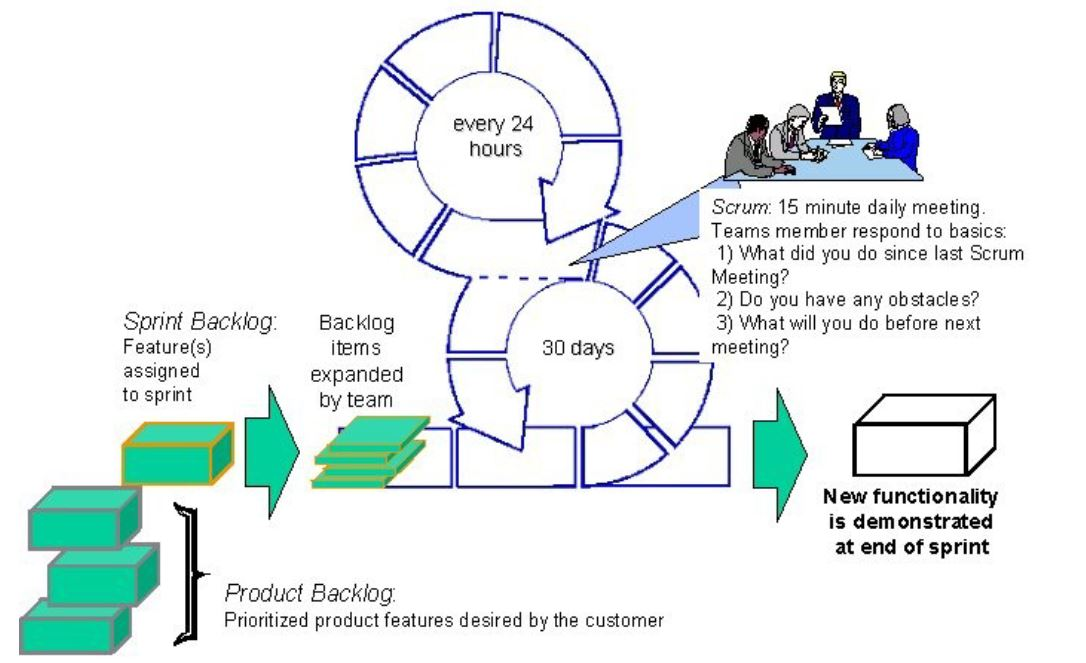
\includegraphics[width=0.95\textwidth]{img/scrum.jpg}
	\end{center}
\end{minipage}
\begin{minipage}{0.3\textwidth}
	Durante lo sprint c'è un daily meeting della durata di 15 minuti in cui si discute l'avanzamento dei lavori locale (ovvero cosa si è fatto ieri e cosa si farà oggi). Inoltre, se qualcuno ha incontrato problemi svolgendo dei work item deve segnalarlo.
\end{minipage}

\begin{itemize}
\item Gruppi che si auto-organizzano
\item Il prodotto evolve attraverso "sprint" mensili (o comunque di durata fissa)
\item I requisiti sono trattati come elementi di una lista detta "product backlog"
\item Non vengono prescritte particolari pratiche ingegneristiche
\item Si basa sull'attività empirica cioè la conoscenza si basa sull'esperienza e  le decisioni si basano su ciò che si è conosciuto
\item Processo iterativo e incrementale per ottimizzare il controllo dello sviluppo e il controllo del rischio
\end{itemize}

\subsubsection*{Sprint}
I progetti Scrum progrediscono attraverso una serie di "sprint", analoghi alle iterazioni della extreme programming (altra pratica agile). Hanno una durata tipica di 2-4 settimane costante, poiché favorisce un ritmo migliore.\\
Durante lo sprint il prodotto viene progettato, realizzato e testato, e durante questo si celebrano tutti gli eventi.\\
\textbf{Non si cambia durante lo sprint:} è necessario che lo scrum master tenga i cambiamenti fuori dallo sprint. Nonostante lo sprint backlog possa essere modificato e rinegoziato tra team di sviluppo e product owner, la durata dello sprint assicura che il rischio di spostarsi da quanto richiesto sia limitato alla durata dello sprint. Uno sprint può essere cancellato se l'obiettivo dello stesso diventa obsoleto, tuttavia ha poco senso vista la durata limitata.

\subsection{Ruoli}
\subsubsection*{Product Owner}
\begin{itemize}
	\item Definisce le caratteristiche del prodotto
	\item Rappresenta il desiderio del committente
	\item Decide date e contenuto del rilascio
	\item È responsabile della redditività del prodotto (ROI)
	\item Definisce le priorità delle caratteristiche del prodotto in base al valore di mercato che gli attribuisce
	\item Adegua le caratteristiche e la priorità ad ogni iterazione, secondo quanto necessario
	\item Responsabile che il Product Backlog sia chiaro e ordinato
	\item Accetta o rifiuta i risultati del lavoro
\end{itemize}

\subsubsection*{Scrum Master}
\begin{itemize}
	\item Rappresenta la conduzione del progetto
	\item Responsabile dell’adozione dei valori e delle pratiche Scrum
	\item Rimuove gli ostacoli 
	\item Si assicura che il gruppo di lavoro sia pienamente operativo e produttivo
	\item Favorisce una stretta cooperazione tra tutti i ruoli e le funzioni
	\item Protegge il gruppo di lavoro da interferenze esterne
	\item Servant leader: aiuta Product Owner e Team di sviluppo condividendo la gestione e le decisioni con il team
\end{itemize}

\subsubsection*{Development Team}
\begin{itemize}
	\item Tipicamente 5-9 persone
	\item Responsabili di realizzare l’incremento in conformità con la Definition of Done
	\item Competenze trasversali (cross functional): programmatori, tester, progettisti di user experience, etc.
	\item Membri di progetto dovrebbero lavorare full-time
	\item Il gruppo di lavoro si auto-organizza: idealmente niente titoli, ma in rari casi può essere una possibilità
\end{itemize}

\subsection{Eventi}
\subsubsection*{Sprint Planning}
Evento time boxed (circa 8 ore per sprint di un mese). L'oggetto di questo è far selezionare dal team di sviluppo gli item da inserire nello sprint backlog, presi dal product backlog. Ciascun task inserito viene quindi stimato (1-16 ore).

\subsubsection*{Daily Scrum}
Detto anche stand up meeting o mischia quotidiana, deve durare al massimo 15 minuti. Non serve a risolvere problemi, ma per sincronizzarsi su quanto fatto e pianificare la giornata per il raggiungimento dello sprint goal. Si aggiorna quindi la scrumboard. Aiuta ad evitare altre riunioni non necessarie.\\
I problemi emersi verranno discussi successivamente con i singoli interessati.\\
\textbf{NB:} non è un SAL (Stato Avanzamento Lavori) per lo scrum master, sono impegni assunti tra pari (team di sviluppo).

\subsubsection*{Sprint Review}
Evento time boxed (circa 4 ore per sprint di un mese).
Il gruppo di lavoro presenta ciò che ha realizzato durante lo sprint tipicamente in forma di demo delle nuove caratteristiche o dell'architettura sottostante (\underline{niente slide,} \underline{max 2 ore per la preparazione}).
Partecipa tutto il gruppo e sono invitati anche gli esterni.

\subsubsection*{Sprint Retrospective}
Evento time boxed (circa 3 ore per sprint di un mese). Si celebra dopo la Sprint Review e prima del prossimo Sprint Planning. Si valuta ciò che sta funzionando e ciò che non sta funzionando:
\begin{itemize}
	\item come migliorare il prodotto?
	\item la Definition of Done è appropriata?
	\item come posso migliorare il prossimo sprint?
\end{itemize}
Vi partecipa tutto il gruppo.
%\newpage
\subsection{Artefatti}
\subsubsection*{Product Backlog}
Raccoglie i requisiti, le funzionalità, i miglioramenti e i fix da realizzare nei prossimi rilasci, essenzialmente una lista di tutti i "desiderata" espressa in modo che sia comprensibile da tutti gli utenti del prodotto o per gli utenti. Le priorità vengono assegnate dal product owner, mentre le stime sono fatte dal development team. Le priorità sono rivalutate all'inizio di ogni sprint, è quindi una lista dinamica che evolve con il prodotto, con un raffinamento continuo.

\subsubsection*{Sprint Backlog}
Ogni componente del Development Team si sceglie qualcosa da fare, il lavoro non è mai assegnato. La stima del lavoro rimanente è aggiornata ogni giorno nel daily scrum, infatti ogni membro del gruppo può modificare parti dello sprint backlog.
Se il lavoro non è chiaro, definire un elemento dello sprint backlog con una stima temporale più ampia, e decomporlo successivamente, aggiornando il lavoro rimanente man mano che diventa più chiaro.

\subsubsection*{Sprint Goal}
Una breve indicazione dell'obiettivo principale dello Sprint. Alcuni esempi:
\begin{itemize}
	\item Database Application: Fare girare l’applicazione anche su SQL Server oltre che su Oracle
	\item Financial Services: Supportare più indicatori tecnici di quanto faccia ABC con dati in tempo reale
\end{itemize}

\subsubsection*{Definition of Done}
Definisce il significato di "svolto" per uno sprint item, ovvero il minimo set di attività per definire che un'attività è completa. Può variare per gruppo di lavoro e dev'essere ben chiara a tutti i membri. È utilizzato per verificare se un'attività è da ritenersi completata.

\subsubsection*{Acceptance Criteria}
Permette di confermare se la storia è completa e funziona come voluto. Sono un insieme di frasi semplici condivise da Product Owner e Development Team. Possono essere incluse con la User Story e rimuovono l’ambiguità dei requisiti.\\
\textit{Esempi}: A user cannot submit a form without completing all the mandatory fields; Information from the form is stored in the registrations database; An acknowledgment email is sent to the user after submitting the form.

\subsubsection*{Sprint burndown chart}
\begin{minipage}{0.6\textwidth}
\begin{center}
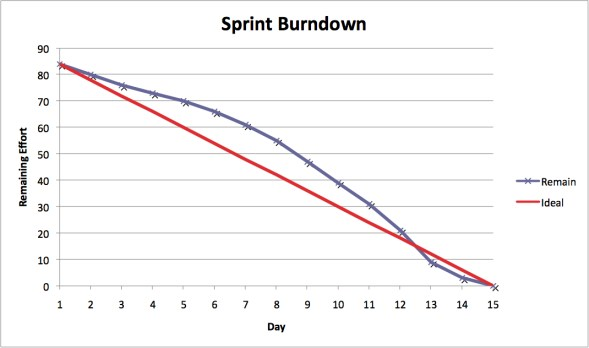
\includegraphics[width=0.95\textwidth]{img/sprint_burndown.jpg}
\end{center}
\end{minipage}
\begin{minipage}{0.4\textwidth}
La linea rossa è la stima, quella blu l'andamento reale. È comune che all'inizio si vada peggio del previsto, tuttavia è facile che poi si vada sotto la stima e si finisca in tempo.
\end{minipage}

\section{Git}
Git è un software di controllo versione distribuito utilizzabile da interfaccia a riga di comando, creato da Linus Torvalds nel 2005.

\subsection{Caratteristiche}
\begin{itemize}
    \item Branching and merging: favorisce lo sviluppo isolato
    \item Piccolo e veloce: la maggior parte delle operazioni viene fatta in locale, solo la condivisione in remoto richiede connessione. È stato realizzato in C per essere leggero e veloce.
    \item Distribuito: ci sono backup multipli della repository creati tramite la \textit{clone}
    \item Integrità: ogni commit è identificato da un ID (checksum SHA-1 di 40-caratteri basato sul contenuto di file o della struttura della directory). Non è possibile cambiare un commit senza modificare l’ID del commit stesso e di i commit successivi.\\
    I commit fanno sempre riferimento al commit padre (il precedente, quello da cui sono cominciate le modifiche).
    \item Staging area: È stata aggiunta un’area di staging dove vengono validati i file modificati che potranno essere versionati con un commit
    \item Free and open source: licenza GNU/GPL 2.0, sorgente gestito su github in repo pubblica.
\end{itemize}
Git salva le variazioni ai file sotto forma di istantanee, non diff. Infatti, ogni volta che si esegue un commit viene fatto uno snapshot dello stato attuale del file system. Inoltre, se un file non subisce modifiche questo sarà un puntatore alla versione precedente, in modo da risparmiare spazio.

\subsection{Aree locali - Stato di un file}
\begin{minipage}{0.4\textwidth}
    In GIT i file della copia locale possono essere:
    \begin{itemize}
        \item Nella \textit{Working directory}, checked out, modificati ma non ancora validati (\textbf{Modified})
        \item Nella \textit{Staging Area}, validati ma non ancora committati. Il commit salva uno snapshot di tutti i file presenti nella staging area (\textbf{Staged})
        \item Nel \textit{Repository locale} (\textbf{Committed})
    \end{itemize}
    Un file appena creato è nello stato di \textbf{Untracked}.
\end{minipage}
\begin{minipage}{0.6\textwidth}
    \begin{center}
        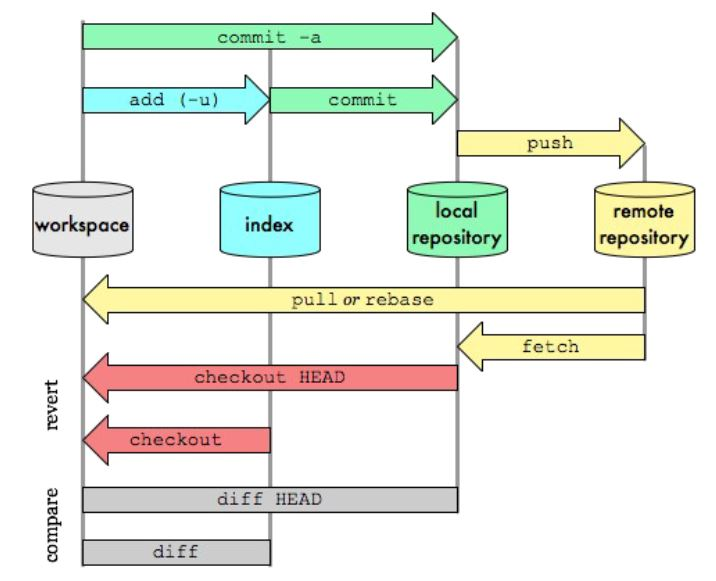
\includegraphics[width=\textwidth]{img/git_command.jpg}
    \end{center}
\end{minipage}

\subsection{Configurazione}
È richiesta una configurazione iniziale dove vengono impostati l’username e l’email da usare per ogni commit:
\begin{itemize}
    \item \verb|git config --global user.name "Bugs Bunny"|
    \item \verb|git config --global user.email bugs@gmail.com|
\end{itemize}
Ci sono tre livelli di visibilità per il config: system (tutti gli utenti), global (utente corrente), local (default, singola repository).
È possibile invocare \verb|git config --list| per avere la lista di tutte le configurazioni.\\\\
Per creare una repository locale si usa \verb|git init| dentro la cartella di un progetto esistente. Tutti i file sono quindi untracked. Viene creata una cartella \verb|.git| contenente la repo.\\
È inoltre possibile clonare una repository remota con \verb|git clone <url>| o locale \verb|git clone <local_directory_path>|.

\subsection{Altri comandi utili}
\begin{itemize}
    \item \verb|git reset HEAD <file_name>|: rimuove un file dalla staging area senza perdere le modifiche
    \item \verb|git checkout -- <file_name>|: rimuove un file dalla staging area perdendo le modifiche
    \item \verb|git status|: vedere lo stato dei file workspace o nella staging area
    \item \verb|git diff|: per vedere cos’è stato modificato ma non ancora validato nella staging area
    \item \verb|git diff --cached|: per vedere cos’è stato modificato nella staging area
    \item \verb|git log|: mostra la lista dei cambiamenti (commit) nel repository locale
    \item \verb|git log -2|: mostra ultimi due commit
    \item \verb|git branch <name>|: crea un nuovo branch indipendente
    \item \verb|git branch|: lista dei branch
    \item \verb|git checkout <branch_name>|: cambia branch su cui si sta lavorando
    \item \verb|git checkout master -> git merge <branch_name>|: effettuare attività di merge di un branch nel master
    \item \verb|git remote|: lista dei repository remoti collegati (possono essere multipli)
    \item \verb|git fetch origin|: recupero i nuovi branch e le modifiche dal remoto senza aggiornare la working copy (senza fare merge)
    \item \verb|git pull origin master|: recupero le ultime modifiche dal repository remoto e aggiorno la working copy (fetch and merge)
    \item \verb|git push origin master|: inviare le modifiche al repository remoto
\end{itemize}

\subsection{SVN vs GIT}
SVN sta per \textit{subversion}. La principale differenza è che il primo è centralizzato, il secondo distribuito.
Inoltre, in SVN una repository può contenere diversi progetti, questo perché il branching avviene sulle singole cartelle, non nella root. In git questo non è possibile, esiste una repo per ogni progetto.\\
Un'altra importante differenza è che in assenza di connessione, in SVN non è possibile continuare il lavoro di versionamento, visto che il database è singolo e centralizzato.


\end{document}